\section{XACML Policy Refactoring Process} \label{sec:approach}
This section describes our approach of refactoring access control policies to improve performance by reducing the number of policy rules. 
For refactoring policies in a systematic way, we propose seven policy splitting criteria
based on attribute set. Moreover, we explain how to select the splitting criterion, which preserves the synergy requirement in the access control architecture. 

 


\subsection{Definition of Policy based Splitting Criteria} \label{subsec:SplittingCriteria}


Given a request, a PDP adopts brute force searching to find its decision
by evaluating the request against policy rules one by one until the PDP finds an evaluation decision.
For request evaluation processing, not of all the rules are applicable to the request.
In order words, only part of the rules (i.e., relevant rules) are applicable to the request and can contribute
to determine a final authorization decision.
We propose an approach to evaluate a request against only the relevant rules for a given request by refactoring
access control policies.
  
%Our approach is to split a single global policy into multiple policies based on attributes combination. 
Our approach refactors a policy into a set of sub-policies where the rules have the same values of attributes of subject, resource, or 
action.
Formally, our approach refactors an policy \normalsize $P$ into 
multiple policies \normalsize $P_{SC_{w}}$ based on Splitting Criteria $SC_{w}$.
These multiple policies contain less number of rules (compared to the number of rules in \normalsize $P$) and conforms to a Splitting Criteria $SC_{w}$. An $SC_{w}$ defines the set of attributes, which classify all of policy rules into subsets with the same attribute values for
selected attributes.
$w$ denotes the number of attributes that have to be considered conjointly for aggregating 
rules based on selected attributes. 


 
We first consider two attributes (e.g., $\langle Subject, Action\rangle$ or $\langle Action$, $Resource\rangle$) for Splitting Criteria. In such a setting, our approach refactors a policy into a set of 
policies each of which rules include the same couple of attribute elements. For example, $\langle Subject, Action\rangle$ criterion
classifies rules with same subjects and actions into sub-policies.
We also extend our Splitting Criteria by considering three attributes such as resource, action, and subject.
Table~\ref{table1} shows our proposed splitting criteria categories according to the attribute elements combination.

\begin{table}[h!]
\centering
\setlength{\extrarowheight}{6 pt}
\begin{tabular}{|>{\small}c|>{\small}c|} 
\hline  \rowcolor{black} 
\bf
\textcolor{white}{Categories}& \bf \textcolor{white}{Splitting Criteria}\\ \hline
$SC_{1}$& {$\langle Subject \rangle, \langle Resource\rangle, \langle Action\rangle$}\\ \hline
$SC_{2}$& {$\langle Subject,Action \rangle, \langle Subject,Resource\rangle$}\\&{$\langle Resource,Action\rangle$}\\  \hline
$SC_{3}$& {$\langle Subject,Resource,Action\rangle$}\\ \hline
\end{tabular}
\caption{Splitting Criteria}
\label{table1}\end{table}



After the splitting process is performed, our approach creates one or more (PDPs) that comply with a certain splitting criterion.
We use SUN PDP \cite{sunxacml} that evaluates requests against the policies specified in XACML.
During request evaluation, SUN PDP checks the request against the policy and determines whether its authorization
decision is permit or deny. Given a request, our approach fetches a SUN PDP loaded with the relevant policy, which is used during the decision making process. Once the applicable policy. The PDP then retrieve the applicable rules that are applicable to the request.


Figure \ref{requestevaluation} presents our approach to handle request evaluation with multiple policies. 
During the evaluation process, given a request, our approach verifies the matching between the request's attributes
and the policy set attributes. Our approach then selects only relevant policy among all of policies for a given request.
After the selection of the relevant policy, all of its relevant rules for the decision making are evaluated.

\begin{figure}[!h]
\begin{center}
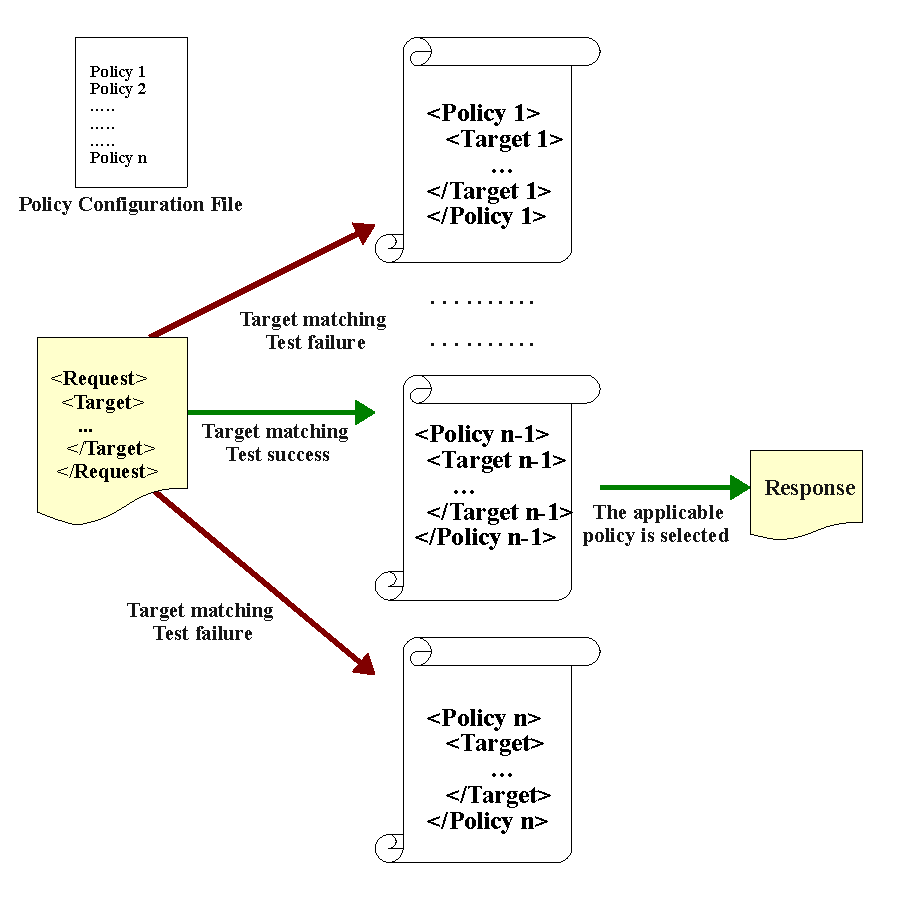
\includegraphics[width=3in, height=3in]{requestevaluation}
\caption{Applicable policy Selection}
\label{requestevaluation}
\end{center}
\end{figure}

Figure \ref{overallprocess} shows an overview of our approach.
In our approach, the policy splitter component plays a role to refactor access control policies.
Given a single PDP loaded with initial global policy, the policy splitter component conducts automated refactoring process by creating multiple PDPs loaded with XACML policies, which are split from the initial global policy based on user specified SC. 
%Afterwards, the policies are included in the 
%framework that supports our approach. 
If the initial global policy is changed, the policy splitter component is required to conduct refactoring of the policy again to create PDPs with the most recent relevant policies.
Our refactoring approach is safe in the sense that the approach does not impact existing functional aspects in a given
system. 

%For system administration, maintaining and updating the access control policies is completely a standalone and simple
%process. System administrators update an policy frequently and have to manage various dimensions of access control 
%systems such the scalability and maintainability.

\begin{figure}[!h]
\begin{center}
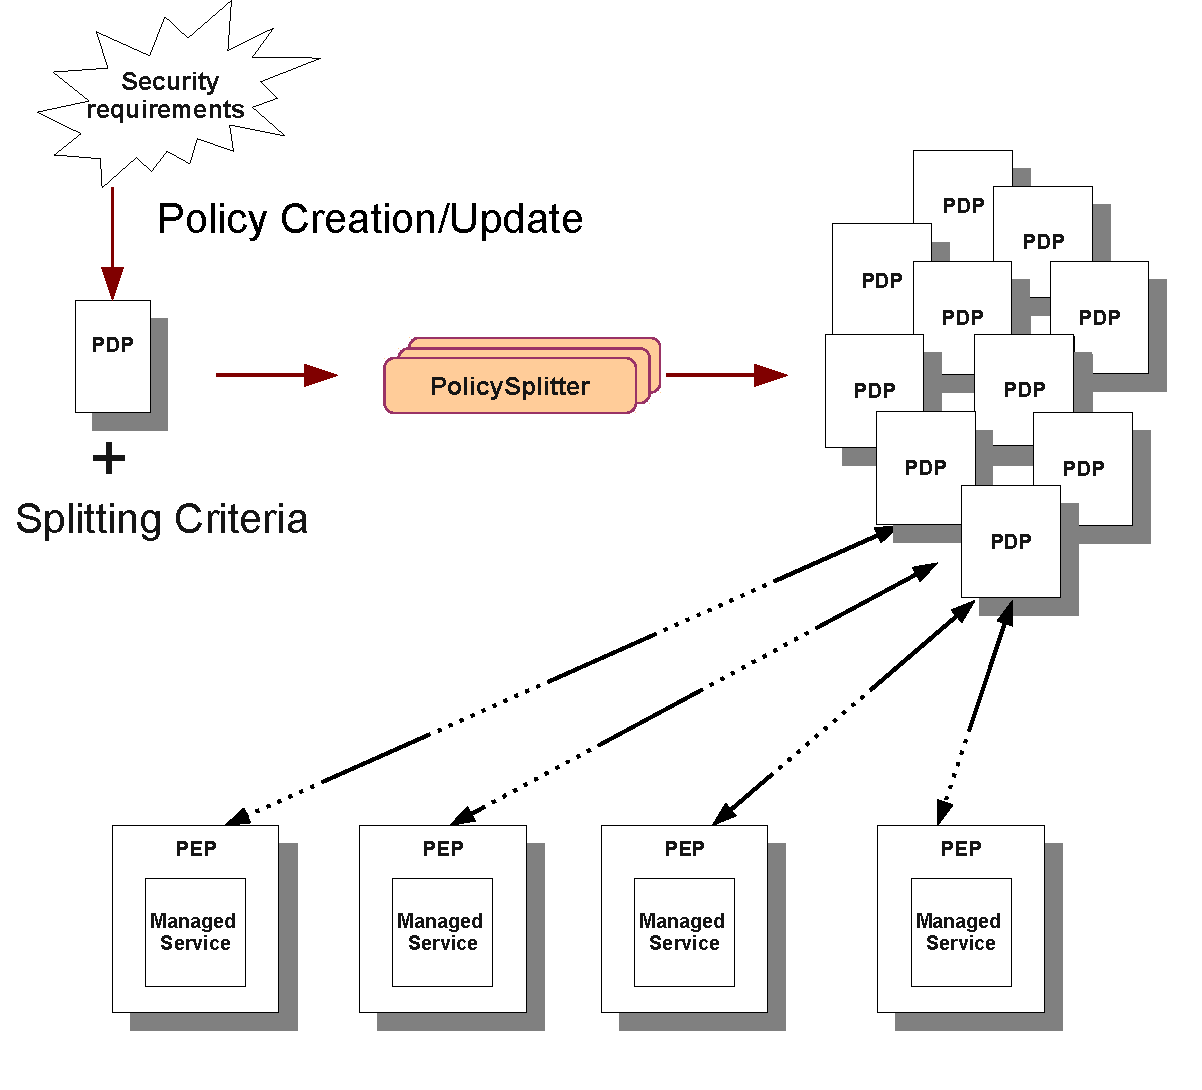
\includegraphics[width=8.5cm, height=8cm]{Overall-process}
\caption{Overview of the Refactoring Process}
\label{overallprocess}
\end{center}
\end{figure} 

To illustrate our approach, we present examples that take into consideration the XACML language features:
\begin{itemize}
\item In Figure \ref{splitting}, our approach refactors an XACML policy $P$  according to the splitting criterion $SC_{1}=\langle Subject\rangle$. Our refactoring results in two sub-policies $Pa$ and $Pb$. Each sub-policy consists of relevant rules with regards to the same subject (Alice or Bob in this case). 

\item
XACML supports multi-valued attributes in policies and requests. In XACML, \CodeIn{Target} elements define a set of attribute values, which match with the context element in 
an access control request. In Figure~\ref{xacml-match}, subject attribute includes two attributes (one is "role" and the other is "isEq-subjUserId-resUserId"). In order to match the subject with multi-valued attributes, a request should include at least \CodeIn{pc-member} and \CodeIn{ture} for "role" and "isEq-subjUserId-resUserId", respectively.
Our approach considers such a whole subject element as a single entity, which is not splitted the policy splitter component.


%\item XACML supports multi-valued attributes in policies and requests. For example, a subject in a given request could be both a manager role and a employee role. We don't consider multi-valued attributes in this paper.


\end{itemize}
\begin{figure}[!h]
\begin{center}
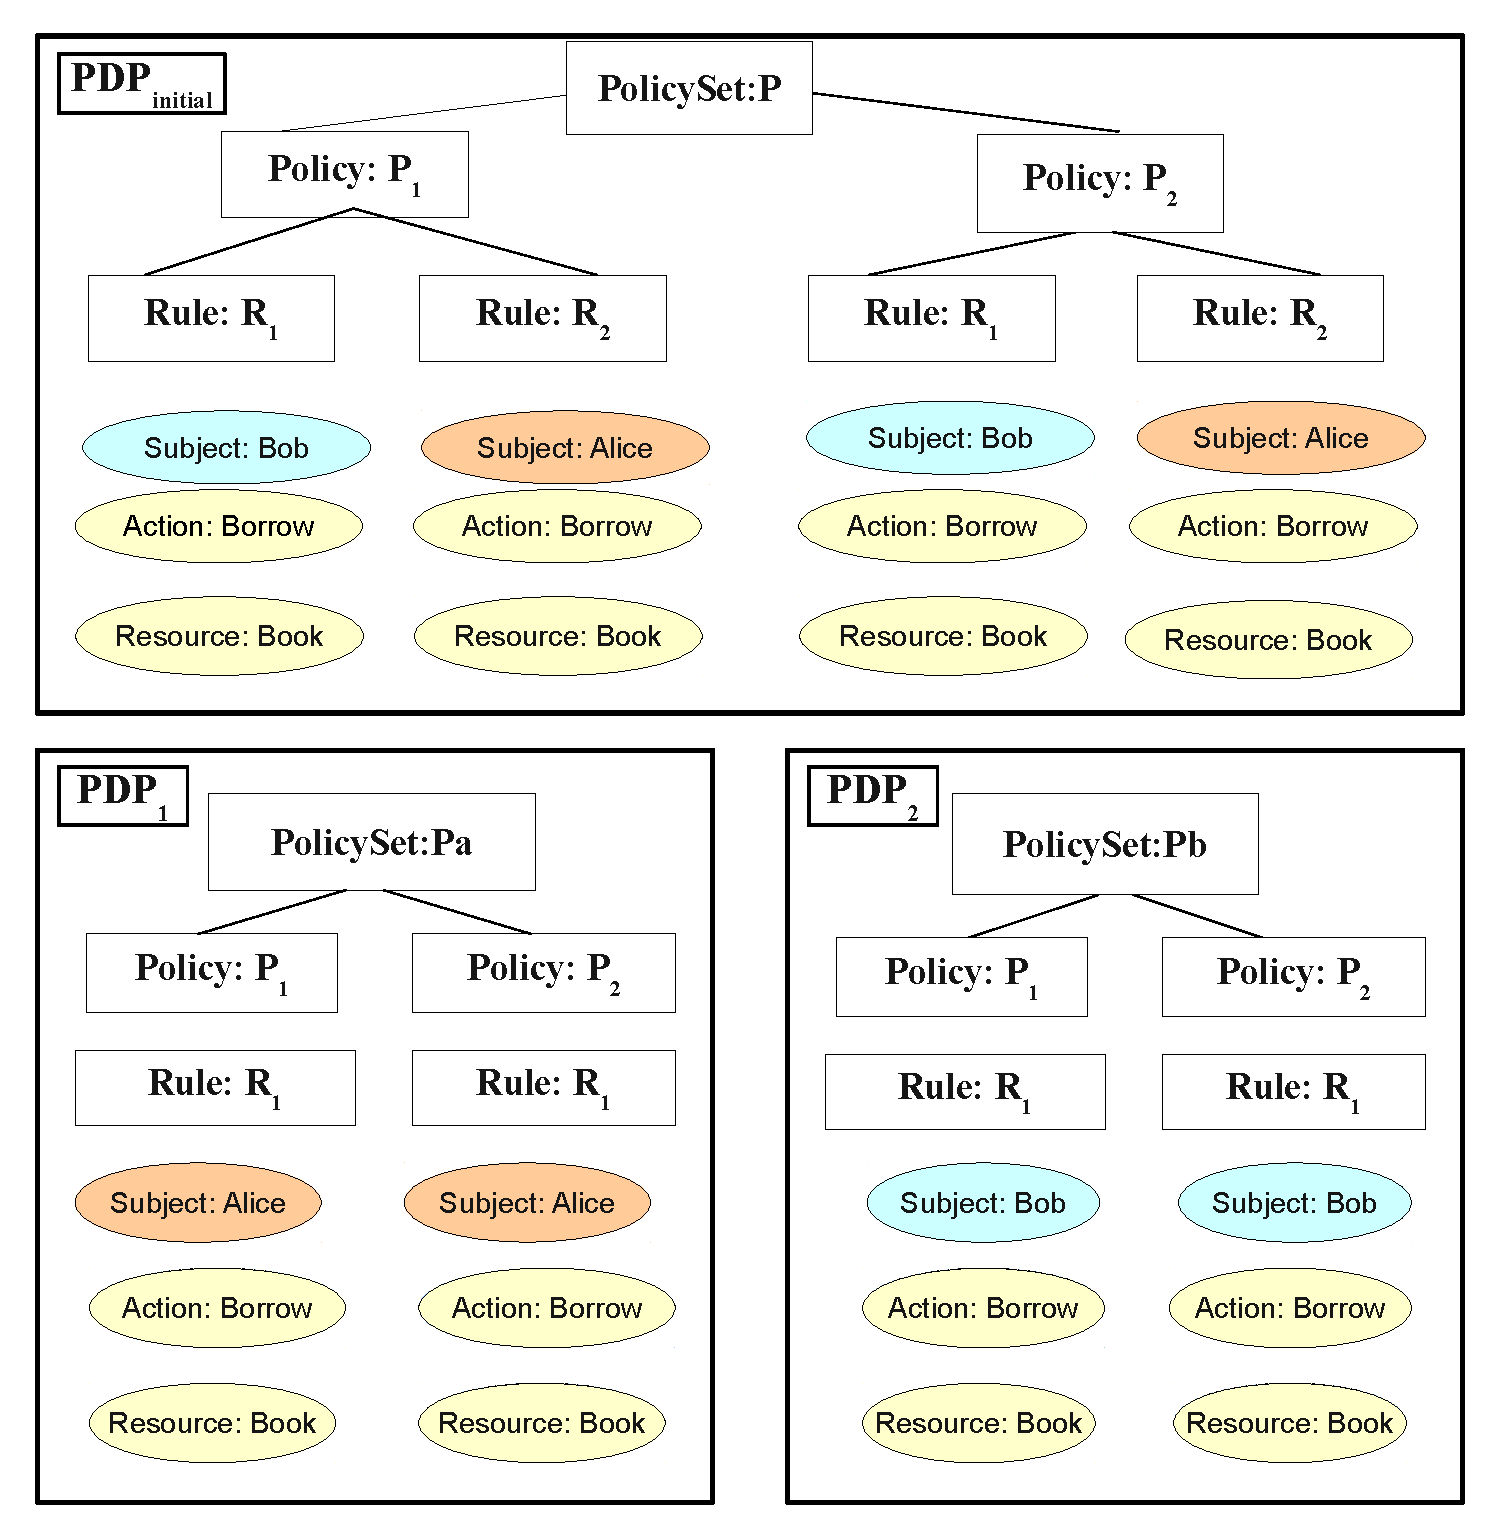
\includegraphics[width=8.5cm, height=7cm]{splitting}
\caption{Refactoring a policy according to $SC_{1}=\langle Subject\rangle$}
\label{splitting}
\end{center}
\end{figure} 


\begin{figure}[!h]
\begin{center}
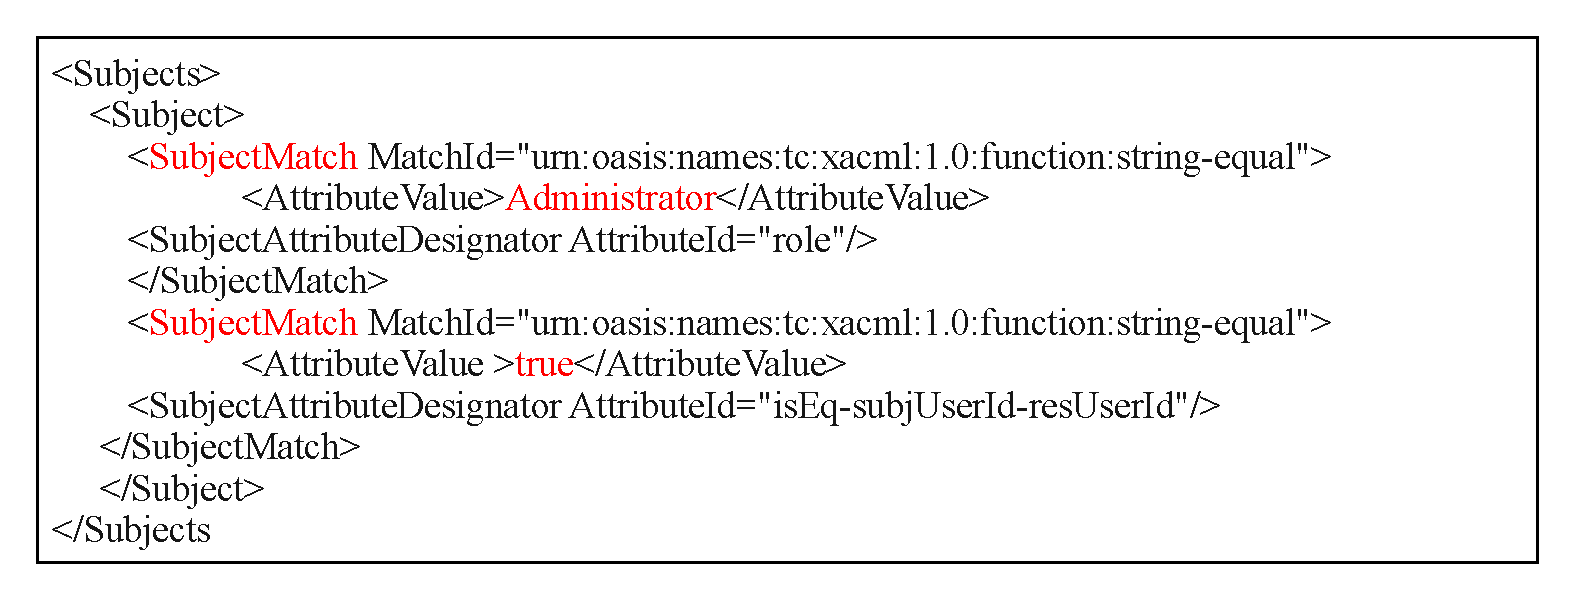
\includegraphics[width=9cm, height=3.5cm]{xacml-match}
\caption{Multi-attributes values in \CodeIn{target} element}
\label{xacml-match}
\end{center}
\end{figure}
 
%Synergy Requirement for Access Control Architecture

\subsection{Architecture Model Preservation: PEP-PDP Synergy}

%We consider the different splitting criteria that we have identified in the previous section.
We propose to preserve the synergy requirement in the access control architecture by mapping a PEP and a PDP loaded
with a relevant policy for a request dynamically at run-time.
As shown in Section~\ref{subsec:SplittingCriteria}, our proposed splitting criteria helps refactoring in access control policies. Given
multiple PDPs after the policy splitting refactoring, we consider (1) how PEPs are organized 
at the application level, and (2) how PEPs are linked to their corresponding PDPs.

In this paper, our goal is to improve performance by reducing request evaluation time. While our approach refactors an initial single PDP into multiple PDPs, this refactoring may not lead to improve performance: a PEP may send its requests to several PDPs.
A PDP, which receives a request is only known at runtime. 
Such a architecture may not reduce evaluation time without PEP-PDP synergy and preserve 
simplicity of the initial architecture model. 
In the best case, the refactoring preserves the simplicity of the initial architecture by keeping a many-to-one association 
between PEPs to PDPs. Given a request, our approach maps a PEP to a PDP with relevant rules for the request.
Threfore, a request issued from a PEP should be handled by the same PDP. Operationally, the request evaluation process involves 
one XACML policy. In this case, our refactoring does not impact the conceptual architecture of the system.

%A deep analysis of the PEPs at the application enables to observe the mapping between the PEPs and the PDP. 
At the application level, the PEP is represented by a method call that triggers a decision making process.
Figure \ref{PEP deployment Example} presents sample PEP code from \cite{legacy}. This code snippets shows an example of a PEP represented by the method \CodeIn{checkSecurity}, which calls the class 
\CodeIn{SecurityPolicyService}, which formulates a request initiates the PDP component.

\begin{figure}[!h]
\begin{center}
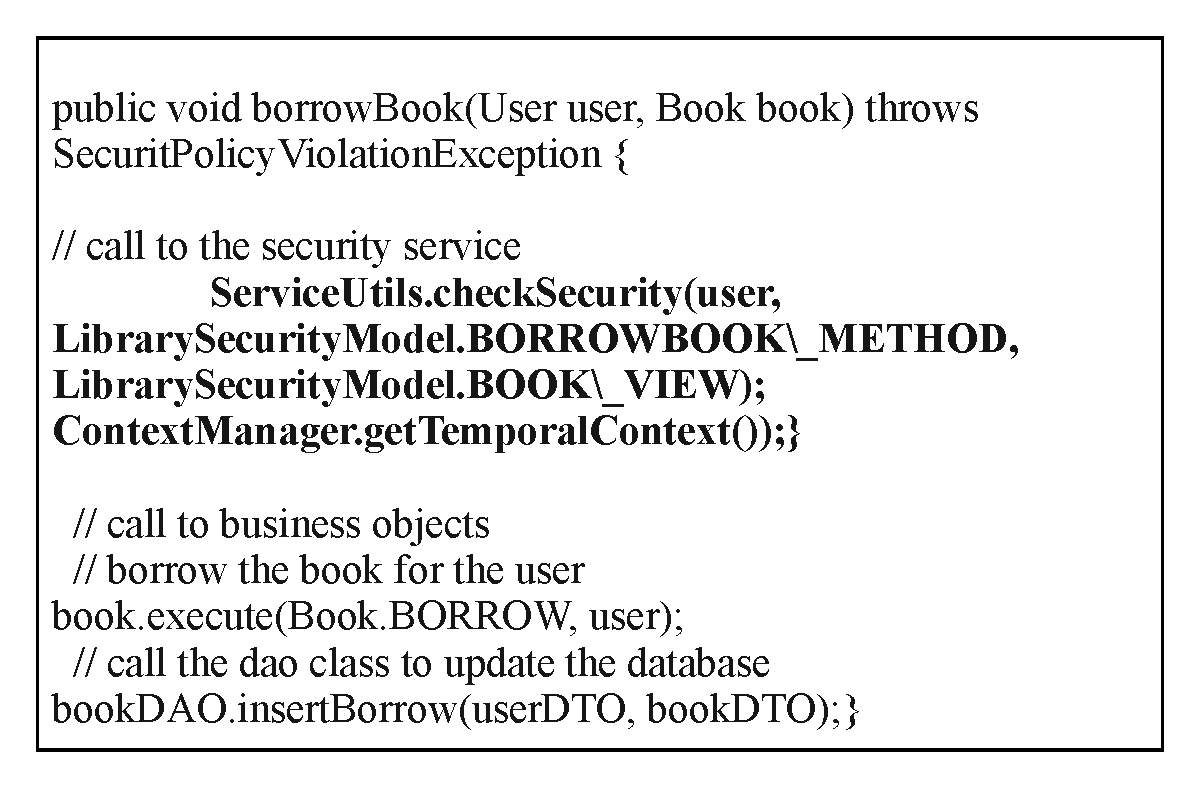
\includegraphics[width=7.5cm, height=4cm]{PEPExample}
\caption{PEP deployment Example}
\label{PEP deployment Example}
\end{center}
\end{figure}

The PEP presented by the method \CodeIn{ServiceUtils.checkSecurity} may issue requests that have subject user role along fixed action and resource (``LibrarySecurityModel.BORROWBOOK\_METHOD''), (``LibrarySecurityModel.BOOK\_VIEW'').
Consider that we refactor a policy using $SC_{2}=\langle Resource,Action\rangle$.
Give a request issued from the PEP, our approach fetches a PDP loaded with a policy containing rules according those action and resource attributes. Depending on the organization of the PEPs in a given application, connecting the rules with their PEPs at the application level may require to identify enforcements points in an application. 


\Comment{
Our empirical results, presented in section~\ref{sec:experiment}, have shown that adopting a policy refactoring based on system functions, as a refactoring strategy, enables to 
have the best splitting criterion in term of performance. 
In this work we consider 3 evaluation studies where the PEPs trigger fixed couples of (action, resource) for variable subjects in the policies, thus the splitting criteria $SC_{2}=\langle Resource,Action\rangle$ is considered as 
the best splitting criteria that enables to preserve the synergy requirement in the architectural model. Inferring automatically the PEPs from the application enables to identify automatically
 for a given application the best splitting criteria, this can be easily applied using the testing technique presented in \cite{legacy}.
}
